
\documentclass{scrartcl} % KOMA Dokumentenklasse mit DIN-Papier als Standard
\usepackage[a4paper]{geometry} % Paket zur flexiblen Anpassung des Seitenlayouts
\savegeometry{default}
\usepackage[autooneside=false]{scrlayer-scrpage} % Paket zur flexiblen Anpassung der Kopf- und Fußzeilen
%
%\usepackage[tocindentauto]{tocstyle} % Paket zur flexiblen Anpassung der Formatierung des Inhaltsverzeichnisses (wird hier nur benötigt, weil einmalig die Nummerierung auf römische Zahlen umgestellt wurde)
 %\usetocstyle{KOMAlike}
%
\usepackage[english]{babel} % Sprachenpaket zur Anpassung der Standardausgaben von bestimmten Schlüsselwörtern und Aktivierung der deutschen Silbentrennung
%
\usepackage{miller}%to intuitively display miller indices%

\usepackage{parskip} %gets rid of hbox warning - just add empty lines to imply linebreaks

\usepackage[utf8]{inputenc} % Kodierungspaket zur Festlegung, wie die eingegebenen Zeichen (Code hier im Dokument) interpretiert werden sollen
%
\usepackage{csquotes}

\usepackage[T1]{fontenc} % Kodierungspaket zur Festlegung, wie die ausgegebenen Zeichen (Buchstaben im PDF-Dokument) implementiert werden sollen
%
\usepackage{lipsum} % Paket zur Einbindung von lateinischen Blindtexten
%
\usepackage{multicol} % Paket zur flexiblen Erstellung mehrspaltiger Texte und zum Zusammenfassen von Spalten in Tabellen
%
\usepackage{ragged2e} % Paket zur Verbesserung der Darstellung von linksbündigem, rechtsbündigem und zentriertem Text (erlaubt Silbentrennung)
%
\usepackage{quoting} % Paket zur ansprechenden Darstellung von Zitaten
%
\usepackage[marginal,norule]{footmisc} % Paket zur flexiblen Anpassung der Formatierung von Fußnoten
%
\usepackage{listings} % Paket zur vereinfachten Einbindung und zur ansprechenden Darstellung von Code in beliebigen Programmiersprachen
%
\usepackage[section, below]{placeins}
%\usepackage[section]{placeins}
%
%
\usepackage{microtype} % Paket zur Verbesserung der Mikro-Typographie durch Anpassung von Zeilenenden und sinnvollen Reduzierung von Silbentrennungen
\usepackage{lmodern} % Schriftenpaket für Latin Modern Schriften (beliebig skalierbare, richtig implementierte Vektorschriften)
%\renewcommand{\rmdefault}{lmss} %to use sans serif by default
\usepackage{textcomp} % Paket zur Erweiterung von verfügbaren Sonderzeichen (Copyright, Trademark, ...)
%
\usepackage{textgreek} %to use greek letters in text
%
\usepackage{amsmath} % Extrem umfassendes Mathematik-Paket der American Math Society
% allow for wider matrices
\newcommand{\tens}[1]{\boldsymbol{\mathsf{#1}}}
\setcounter{MaxMatrixCols}{20}
\usepackage{mathtools} % Erweiterung des amsmath-Pakets (enthält amsmath-Paket)
% Ergänzungen für Mathe:
\DeclarePairedDelimiter\abs{\lvert}{\rvert}%
\DeclarePairedDelimiter\norm{\lVert}{\rVert}%
%
%
% Anpassung von Klammern 
% Swap the definition of \abs* and \norm*, so that \abs
% and \norm resizes the size of the brackets, and the 
% starred version does not.
\makeatletter
\let\oldabs\abs
\def\abs{\@ifstar{\oldabs}{\oldabs*}}
%
\let\oldnorm\norm
\def\norm{\@ifstar{\oldnorm}{\oldnorm*}}
\makeatother
%
%
\usepackage{amsfonts} % Schriftenpaket der American Math Society zur Erweiterung der Schriften in Mathe-Umgebungen
%
\usepackage{amssymb} % Paket zur Erweiterung der verfügbaren Mathe-Symbole
%
\usepackage{MnSymbol} % Paket zur Erweiterung der verfügbaren Mathe-Symbole
%
\usepackage{graphicx} % Paket zur vereinfachten und flexiblen Einbindung von Grafiken (jpg, png, pdf)
%
\usepackage{pdfpages} % Paket zur vereinfachten und flexiblen Einbindung von mehrseitigen PDFs
%
\usepackage{chemformula} %Paket für chem. Formeln e.g. with \ce or \ch and stuff in brackets
%
\usepackage{xcolor} % Farbenpaket zur vereinfachten Einbindung und Anpassung von Farben
%
\usepackage{booktabs} % Paket zur Verbesserung der Darstellung von horizontalen Linien in Tabellen
%
\usepackage{multirow} % Paket zum Zusammenfassen von Zeilen in Tabellen
%
\usepackage{tikz} % Paket zur Erstellung von ansprechenden und anspruchsvollen Zeichnungen innerhalb von LaTeX
%\usepackage{pgfplots} % Paket zur Erstellung von ansprechenden und anspruchsvollen Plots innerhalb von LaTeX
%
\usepackage[style=nature, backend=biber]{biblatex} % Paket zur vereinfachten und automatisierten Erstellung eines Literaturverzeichnisses aus einer externen Datenbank

%
\usepackage{xparse} % Paket zur Erweiterung der Funktionalitäten bei der Definition von neuen Befehlen und Umgebungen
%
\usepackage{hyperref} % Paket zur Erstellung und Anpassung von anklickbaren, intelligenten Querverweisen innerhalb des Dokuments und Hyperlinks (Weblinks, Maillinks, Filelinks)
%
\def\code#1{\texttt{#1}} % to display cod in monospace using \code{arg1}
%
%
%
%
% Einstellungen für das Dokument:
%
 \KOMAoptions{headsepline, footsepline}
 \setkomafont{headsepline}{\color{gray}}
 \setkomafont{footsepline}{\color{gray}}
 \setkomafont{pagehead}{\scshape}
 \setkomafont{pagefoot}{} %\bfseries
 \automark[subsection]{section}
 \lohead{}
 \cohead{\rightmark}
 \rohead{}
 \lofoot{}
 \cofoot{\pagemark}
 \rofoot{}
%
%
\definecolor{meinSchwarz} {RGB} {0,0,0}
%
\hypersetup{linktoc = all, colorlinks ,  citecolor = meinSchwarz , linkcolor = blue, urlcolor  = meinSchwarz , filecolor = meinSchwarz }
%
%\addto\extrasngerman{\def\figureautorefname{Abb.}}
%
\setlength{\parindent}{0pt}
\setlength{\parskip}{0.5\baselineskip plus 0.2\baselineskip minus 0.1\baselineskip}
\linespread{1.25}
%
\newcommand{\degcel}{\,\textcelsius{} }
%
% Angaben zu Variablen
\graphicspath{{graphics}}
\bibliography{pfm_practical.bib}
%

\begin{document}

%
\begin{titlepage}
\begin{center}

\includegraphics[width=0.5\textwidth]{graphics/FAU_TechFak_EN_H_black.eps}

\LARGE Department Materials Science

\Large WW8: Materials Simulation

\LARGE \textbf{Practical: Phase-Field Method}

\Large Basics and Application in Materials Science



\vfil
\Large Leon Pyka (22030137)



\Large \textbf{Supervision: }
\end{center}

\thispagestyle{empty}
%
\end{titlepage}
%

\setcounter{page}{1}

\tableofcontents
\newpage
\section{Introduction}
Phase-field simulation is a versatile application in the toolbox of materials simulation. It is often used for simulations of phase transitions, dislocation evolution, fracture simulations etc. The following practicals aim is to get a practical introduction into the subject. In two separate tasks a 1D single-component solidification simulation, calculation of a bulk energy density coefficient and gradient energy density coefficient are going to be conducted. 

\section{Task 1: 1D Single-Component Solidification} \label{sec:task1}

To simulate a 1D single-component solidification we utilize the following energy density:

\begin{equation}
	F = \int \bigl( f_{0} \phi^{2}(1- \phi)^{2}  + \frac{K_{\phi}}{2} \lvert \nabla \phi \rvert ^{2} \bigr) d \vec{r}
\end{equation}

As soldification is a a non-conservative process, the kinetics are governed by the Allen-Cahn equation (for the  homogeneous, isotropic case).

\begin{equation}
	\frac{\partial \phi}{\partial t} =-L \frac{\delta F}{\delta \phi} \label{eq:alle_cahn_homo_iso}
\end{equation}

Here the functional derivative \(\frac{\delta F}{\delta \phi}\) of an energy functional eq. \ref{eq:energy_functional_general} can be evaluated as eq. \ref{eq:func_derivative_general}.\\


\begin{subequations}
	\begin{align}
		F =& \int f(\vec{r}, \phi, \nabla \phi) d\vec{r} \label{eq:energy_functional_general} \\
		\frac{\delta F}{\delta \phi} =& \frac{\partial f}{ \partial \phi} - \nabla \cdot \frac{\partial f}{\partial (\nabla \phi)} \label{eq:func_derivative_general}
		\end{align}
\end{subequations}

Solving the functional derivative from eq. \ref{eq:alle_cahn_homo_iso} yields:

\begin{subequations}
	\begin{align}
		\frac{\delta F}{\delta \phi} =& 2 f_{0}\phi (1-\phi)^2 + 2 f_{0}\phi^{2} (\phi -1) - K_{\phi} \nabla^{2} \phi \Leftrightarrow \\
		\Leftrightarrow  & 2\phi^{3}  -4\phi^{2} + 2\phi - K_{\phi} \nabla^{2} \phi
	\end{align}
\end{subequations}

Inserting the result into eq. \ref{eq:alle_cahn_homo_iso} results in:

\begin{equation}
	\frac{\partial \phi}{\partial t} = -L \bigl[  f_0 ( 2\phi^{3} -4\phi^{2} + 2\phi) - K_{\phi} \nabla^{2} \phi \bigr]
\end{equation}

As the governing equation for solving the PDE we apply Dirichlet boundary conditions \(\phi_{1} = 0; \phi_{n}=1\) and discretize the partial derivative \(\frac{\partial \phi}{\partial t}\) as:

\begin{subequations}
	\begin{align}
	\frac{\partial \phi}{\partial t}  \approx \frac{\phi_{next} - \phi}{\Delta t} &=  -L \bigl[  f_0 ( 2\phi^{3} -4\phi^{2} + 2\phi) - K_{\phi} \nabla^{2} \phi \bigr] \Leftrightarrow \\
	\Leftrightarrow \phi_{next} & = -\Delta t L \bigl[  f_0 ( 2\phi^{3} -4\phi^{2} + 2\phi) - K_{\phi} \nabla^{2} \phi \bigr]
    \end{align}
\end{subequations}

and \(\nabla^{2} \phi(x) \) is discretized according to the (forward) finite differences scheme:

\begin{equation}
	\nabla^{2} \phi(x_{i}) \approx \frac{\phi(x_{i+2}) - 2\phi(x_{i+1}) + \phi(x_{i}) }{\Delta x^{2}} \label{eq:forward_euler_second_derivative}
\end{equation}

where \(x_{i}\) is the node at which the value is computed and \(\Delta x\) is the node distance. The initial result is plotted in fig. \ref{fig:solidification_init}. As can be seen in \ref{fig:solidification_f0} \(f_{0}\) seems to be reciprocally proportional energy functional over time. With decreasing value the transition region (where \(\phi\) changes from 0 to 1) becomes broader. The opposite effect can be observed in fig. \ref{fig:solidification_K} with variation of \(K_{\phi}\). Additional the energy density functional seems to become broader but only changes its peak value for increased K-values. L does not seem to have any influence on the \(\phi\), the energy or energy density - see fig. \ref{fig:solidification_L} .


\begin{figure}[htb]
	\centering
	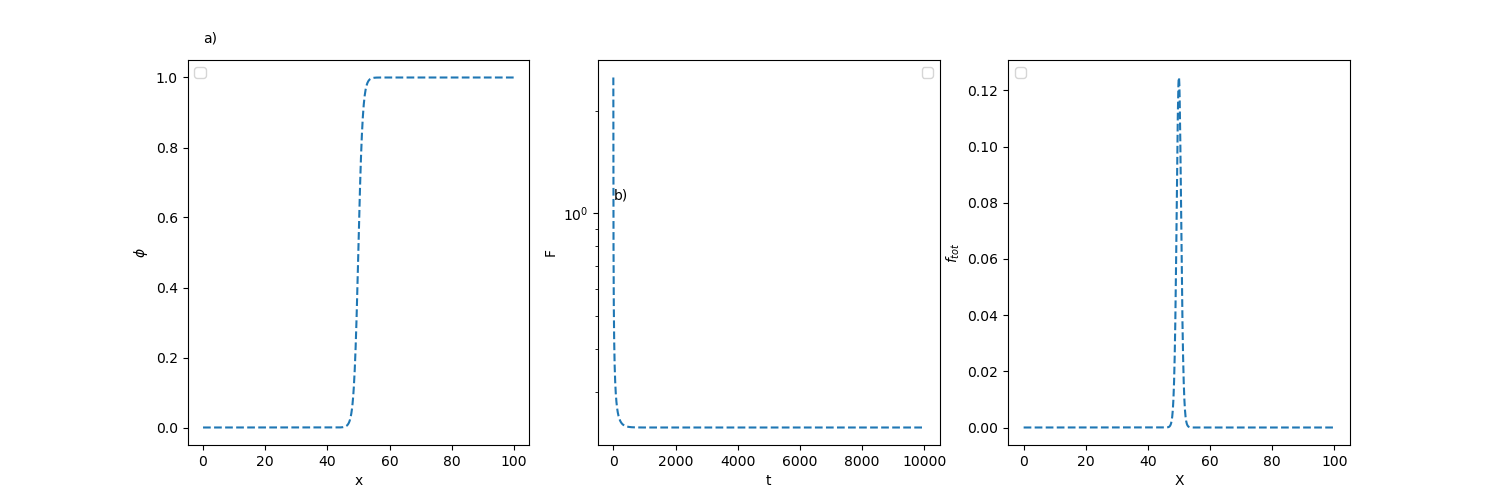
\includegraphics[width=\textwidth]{solidification_initial.png}\label{fig:solidification_init}
	\caption{Initial results of the 1D single-component solidification simulation.}
\end{figure}

\begin{figure}[htb]
	\centering
	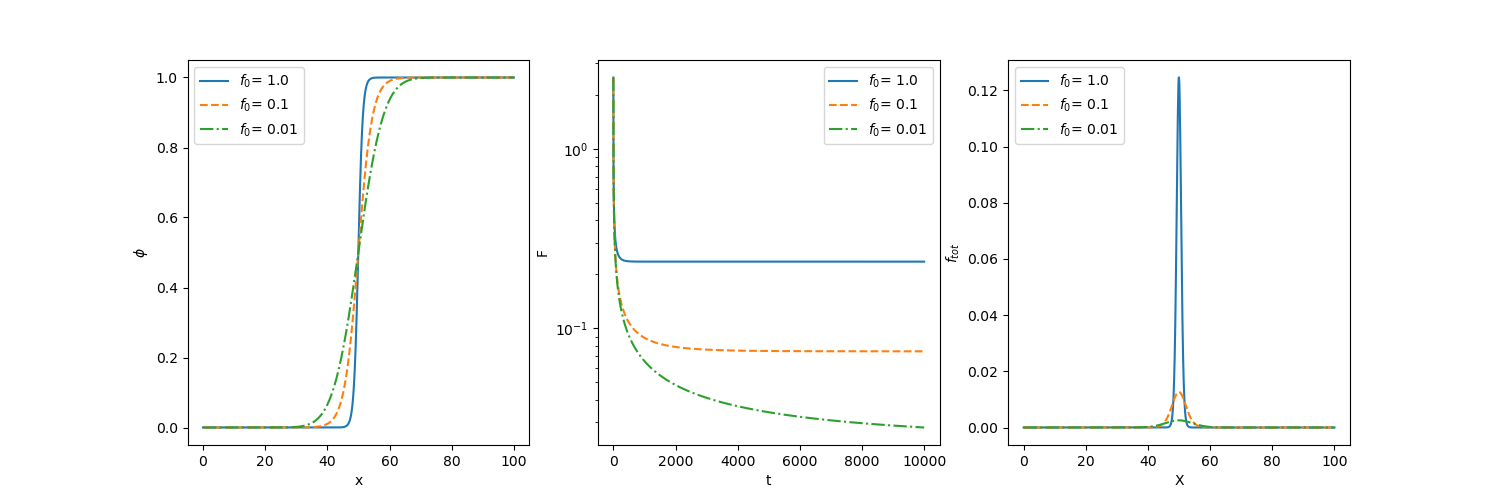
\includegraphics[width=\textwidth]{solidification_vary_f0.png}\label{fig:solidification_f0}
	\caption{Results of the 1D single-component solidification simulation with various \(f_{0}\) values.}
\end{figure}

\begin{figure}[htb]
	\centering
	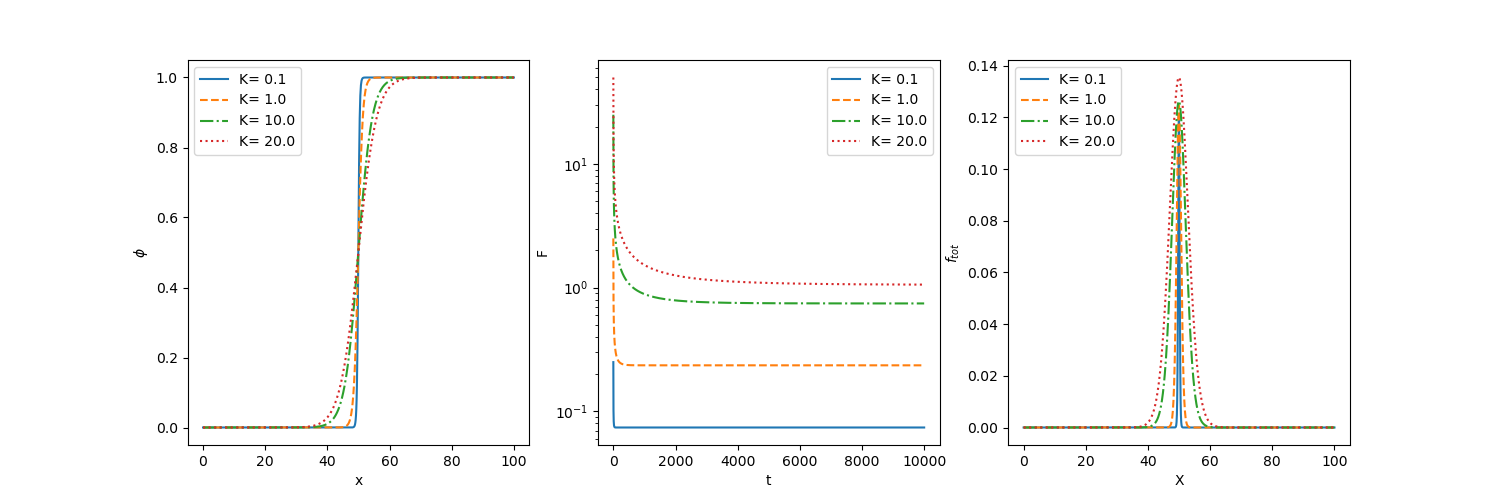
\includegraphics[width=\textwidth]{solidification_vary_K.png}\label{fig:solidification_K}
	\caption{Results of the 1D single-component solidification simulation with various K values.}
\end{figure}


\begin{figure}[htb]
	\centering
	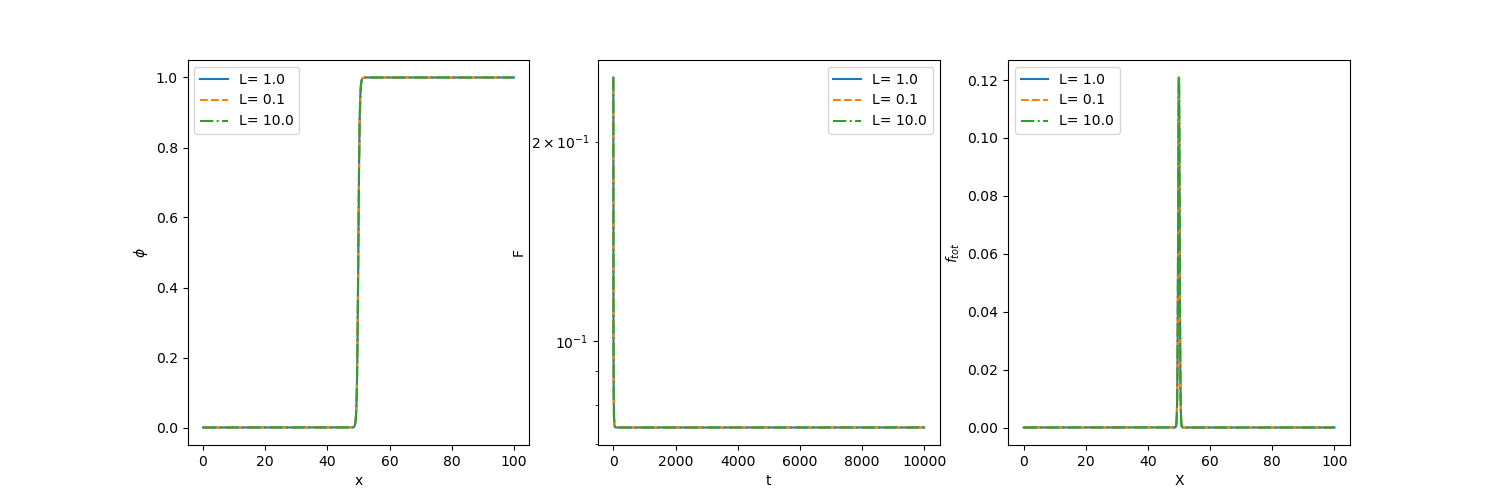
\includegraphics[width=\textwidth]{solidification_vary_L.png}\label{fig:solidification_L}
	\caption{Results of the 1D single-component solidification simulation with various L values.}
\end{figure}

\section{Task 2: Determination of \(f_{0}\)}
The equilibrium Al concentration of the disordered \(\gamma \)-Phase \(c_{\gamma}^{e}\) has been determined to be 0.165 and the  Al concentration of the ordered \(\gamma ' \)-Phase \(c_{\gamma '}^{e}\) has been determined to be 0.230 \cite{zhu2002}. The bulk energy density function is constructed as:

\begin{equation}
	f_{bulk} = f_{0} (c_{\gamma '}^{e} - c)^{2}(c_{\gamma}^{e} - c)^{2} \label{eq:f_bulk_NiAl}
\end{equation}

The \( f_{0}\) needs to be fitted so that it results in an energy gradient of \(\Delta f 149 \frac{\mathrm{J}}{\mathrm{mol}} \) \cite{zaisera}. This is accomplished by choosing the right \(f_{0}\) to reach the right value at the local maximum of eq. \ref{eq:f_bulk_NiAl}. The local maximum of the function can be found automatically by finding the second root of the derivative of eq. \ref{eq:f_bulk_NiAl}:

\begin{equation}
	\frac{df_{bulk}}{dc} = -2 f_{0} (c_{\gamma '}^{e} - c)(c - c_{\gamma}^{e})^{2} + 2 f_{0} (c_{\gamma '}^{e} - c)^{2}(c - c_{\gamma}^{e})
\end{equation}

Using the \code{scipy} package of Python this can be achieved using \code{scipy.optimize.root\_scalar(func, x0=0.2)} where 0.2 is the initial starting point, looking for \(c_{max}\). Here \(c_{max}\) is found at 0.1975. Solving \ref{eq:f_bulk_NiAl} for \(f_{0}\) results in a value of \(\approx 133.6 \cdot 10^{6} \frac{\mathrm{J}}{\mathrm{mol}}\).  The resulting function of the corresponding parameters is plotted in \ref{fig:alni_fitted}.


\begin{figure}[htb]
	\centering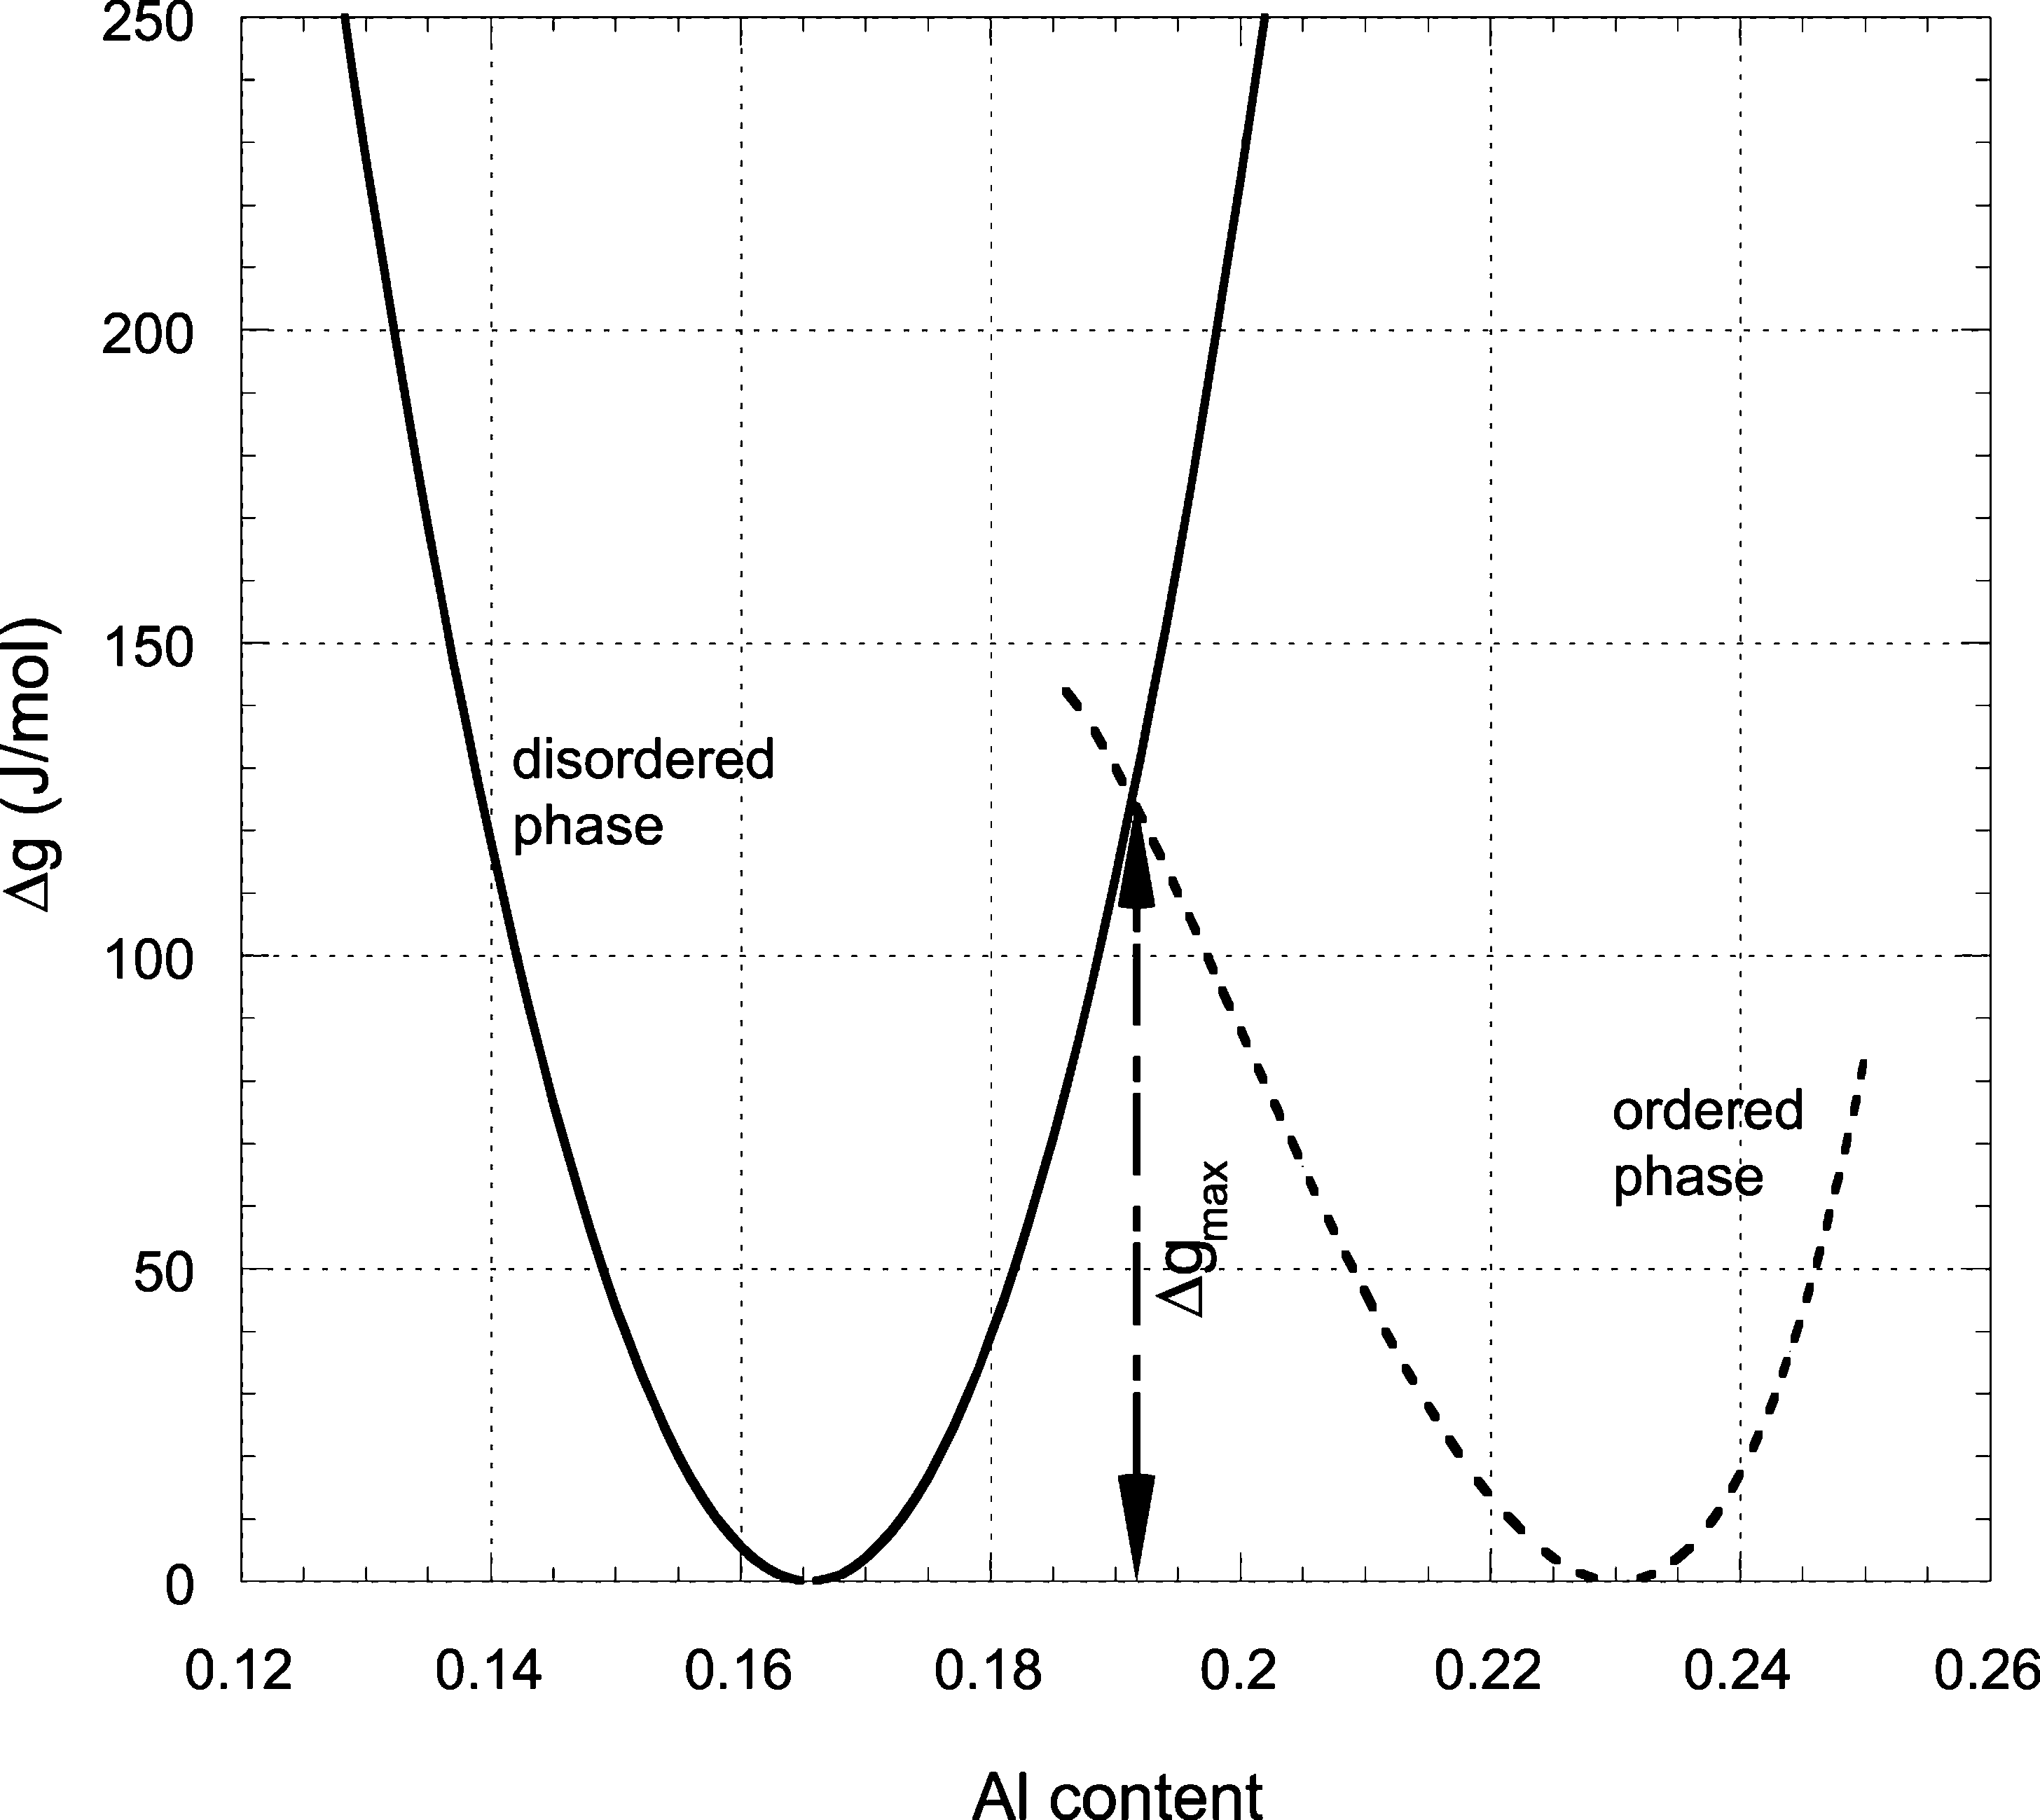
\includegraphics[width=\textwidth]{NiAl_gibbs_free_energy.png}\label{fig:AlNi_gibbs}
	\caption{Calculated chemical free energy as a function of composition for both the disordered and ordered phase at 1300 K reproduced from \cite{zhu2002}.} 
\end{figure}

\begin{figure}[htb]
	\centering
	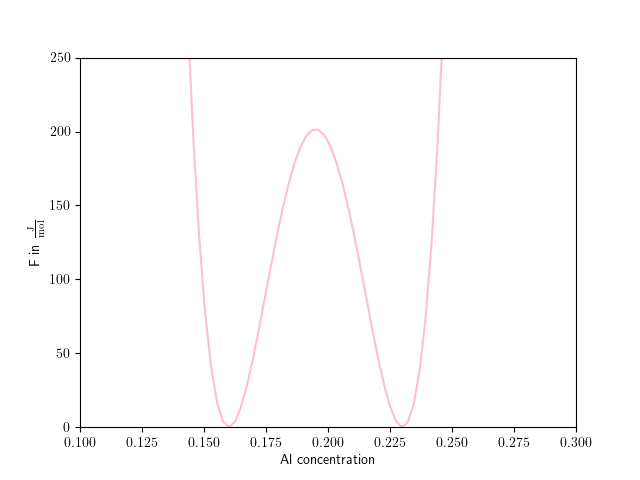
\includegraphics[width=\textwidth]{alni_fitted.png}\label{fig:alni_fitted}
	\caption{Plot of bulk energy of binary NiAl mixture with \(c_{\gamma}^{e} = 0.165\),  \(c_{\gamma '}^{e} = 0.23\) and \(f_{0} = 133.6 \cdot 10^{6} \frac{\mathrm{J}}{\mathrm{mol}} \).}
\end{figure}

\section{Task 3: Determination of \(K_{c}\) }
In this task the gradient energy density coefficient of a binary NiAl-system is calculated. Apart from the governing equation being the Cahn-Hillard equation (eq. \ref{eq:cahn_hillard} ) as we are dealing with a conserved field, the general algorithm is similar to sec. \ref{sec:task1}. 

\begin{equation}
	\frac{ \partial c}{ \partial t} = M \nabla^{2} \frac{\delta F}{\delta c} \label{eq:cahn_hillard}
\end{equation} 

The functional for the binary system is evaluated as follows:

\begin{equation}
	\frac{\delta F}{\delta c} = 2 f_{0}(c_{\gamma '} - c )(c - c_{\gamma})^2 + 2 f_{0} (c - c_{\gamma})(c_{\gamma '} - c )^{2} - K_{c} \nabla^{2} c  \label{eq:functional_NiAl}
\end{equation}
		
\(\nabla^{2}(\cdot)\) is (both in eq. \ref{eq:functional_NiAl} and eq. \ref{eq:cahn_hillard}) is discretized as in sec. \ref{sec:task1} eq. \ref{eq:forward_euler_second_derivative}.  The following coefficients are used molar Volumen \(V_{m} = 10^{-5} \frac{m^{3}}{mol}\), interface mobility \(M = 10^{-17} \frac{mol^{2}}{J m s}\), length segment \(dx = 10^{-8} m\), \(f_{0} = 134 \cdot 10^{6} \frac{J}{mol}\) and a experimental interface energy of \( F_{inte} = 5 \sim 50 \cdot 10^{-3} \frac{J}{m}\). 

As M is function of molar quantity of substance for calculating the energy we have to add define an adjusted \( M_{new} = M * V_{m}^{2}\). Running the simulation for various values of \(K_{c}\) results in fig. \ref{fig:vary_K}. Printing the energies alongside the \(K_{c}\) values shows that to achieve \(F_{ine} < 0.5 \frac{J}{mol}\) we need to use \(K_{c} < 3.5 \cdot 10^{-6} \frac{J}{m}\).

\begin{figure}[htb]
	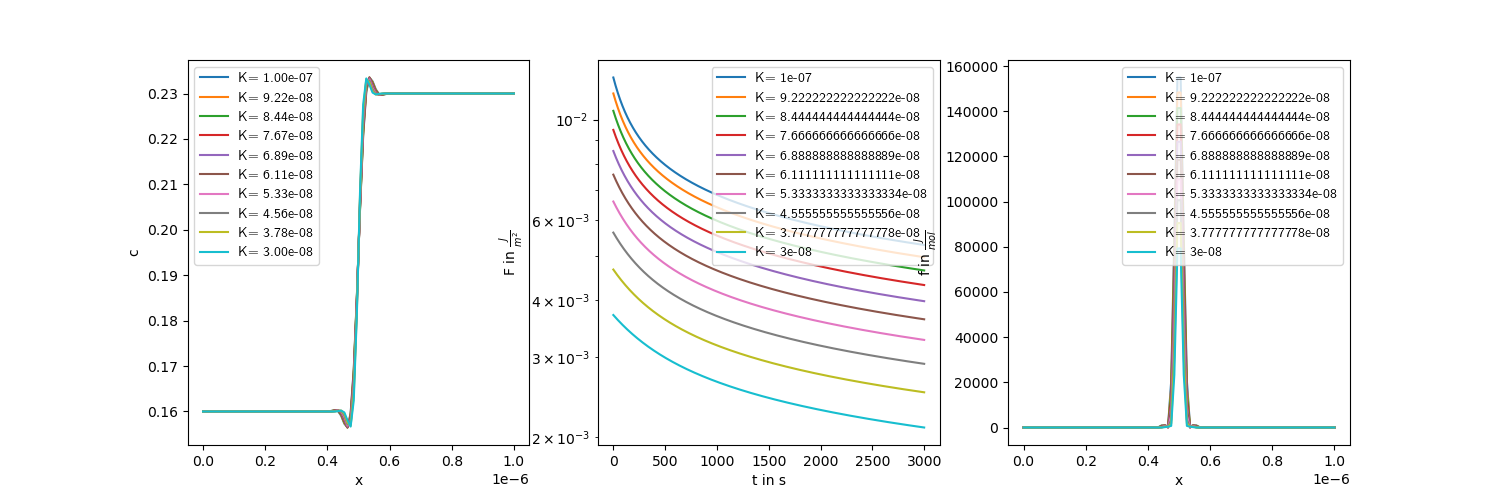
\includegraphics[width=\textwidth]{find_K_grad_energy_density.png} \label{fig:vary_K}
	\caption{Results of the conserved binary NiAl-system simulation with various \(K_{c}\) values.}
\end{figure}

For expanding the calculation of the concentrations we need to implement eq. \ref{eq:forward_euler_second_derivative} in 2D:

\begin{equation}
	\nabla^{2} c_{i,j} = \frac{c_{i,j-1} + c_{i,j+1} - 4c_{i, j} + c_{i-1, j} + c_{i+1, j}}{\Delta x^{2}} 
\end{equation}

where the concentrations are mapped on a \(n \times n\)-Matrix. Running the simulation for 1000\(dt\) results in fig.  . Here we applied an initially random concentration with \(c_{init = 0.195}\) as a mean value for a gauss distributed matrix using the \code{numpy.random.normal(loc=0.195, scale=0.01, size=(N,N))} function. Over time we see, the distribution becomes smooth, while maintaining the composition of several domains of \(\gamma \\ \gamma '\)-Phases.

\begin{figure}
	\centering
	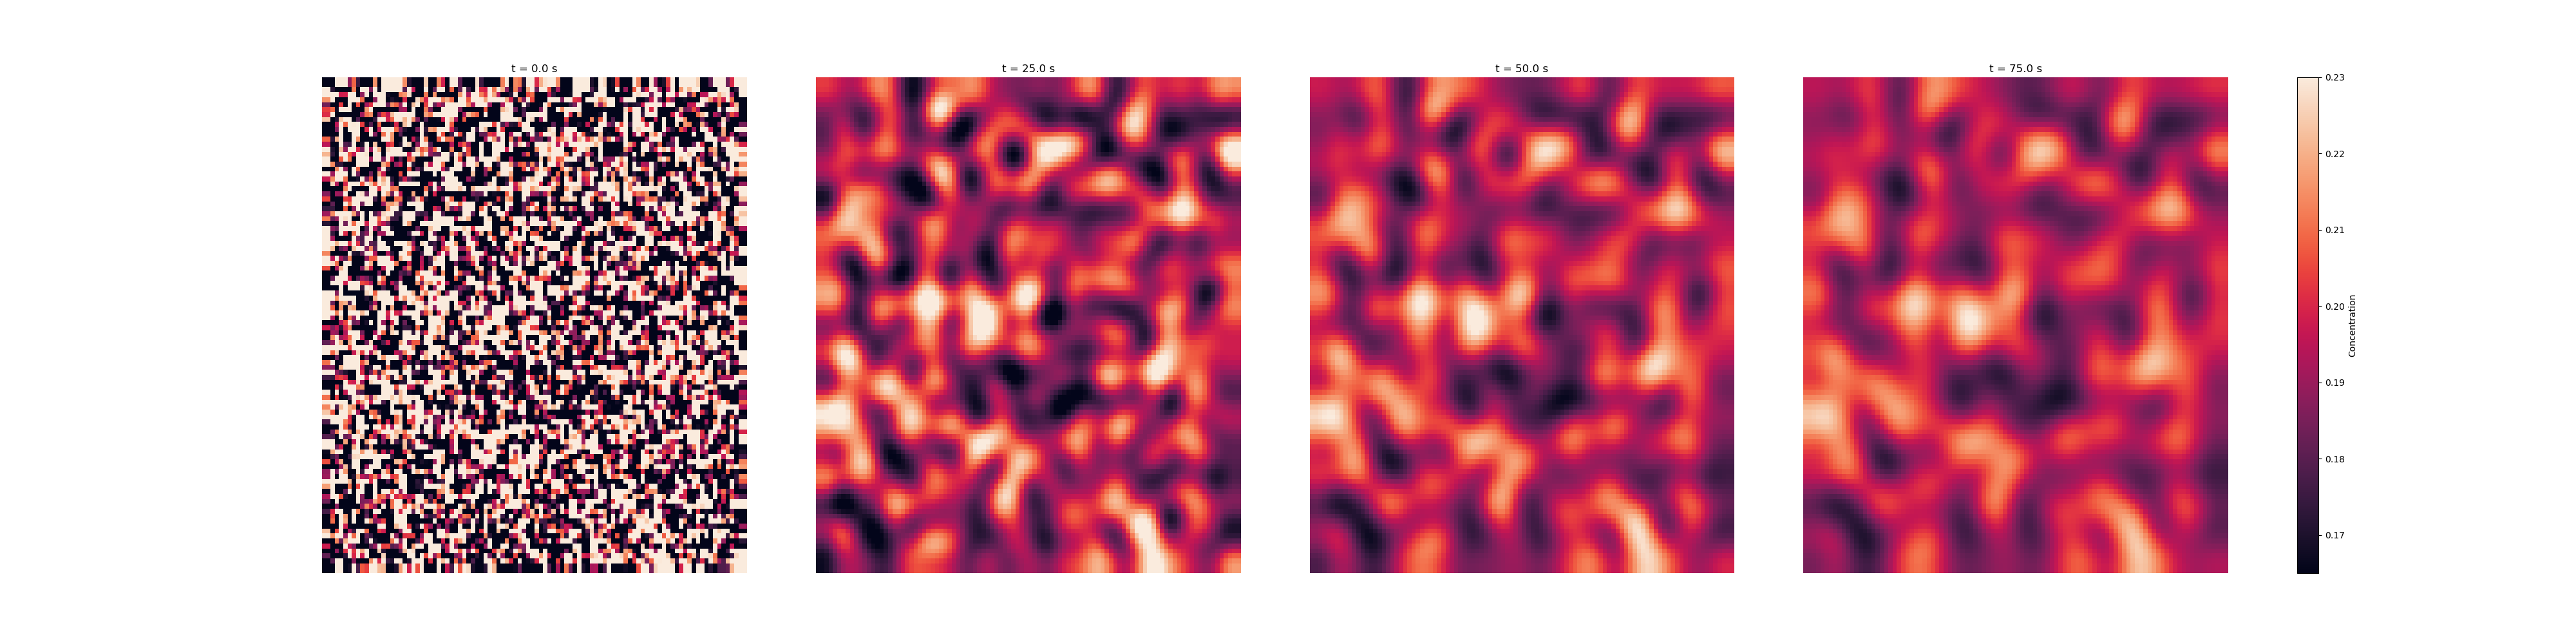
\includegraphics[width=\textwidth]{NiAl_2D.png} \label{fig:NiAl_2D_heatmaps}
	\caption{Heatmaps of concentrations over time calculated by conserved phase-field method from an initially randomly distributed concentration map.}
\end{figure}


%\listoffigures
\printbibliography



\end{document}
